指定したgopathがファイルシステムの普通のディレクトリ名だったとしましょう。当然、自由に一つのディレクトリ名を設定することができます。次にこのパスをGOPATHに追加します。GOPATHは複数のディレクトリを含んでもよいと前にご紹介しました:windowシステムでは環境変数を設定します;linux/MacOSシステムではターミナルに\texttt{export gopath=/home/astaxie/gopath}コマンドを入力するだけです。しかし、gopathというソースディレクトリには3つのディレクトリpkg、bin、srcがあることを保証しなければなりません。作成した新しいプロジェクトのソースコードはsrcディレクトリの下に置きます。現在暫定的に我々のブログディレクトリをbeeblogと呼ぶことにしましょう。下はwindow下での環境変数とディレクトリ構造のスクリーンショットです:

\begin{figure}[H]
   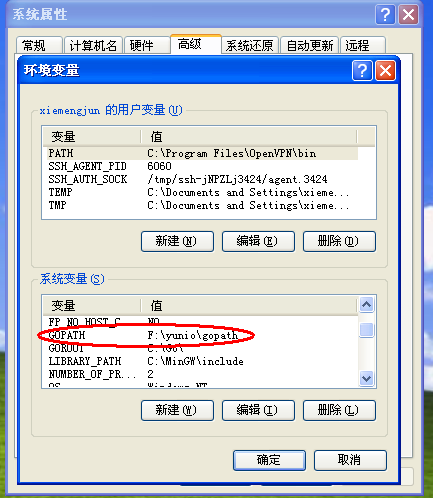
\includegraphics[width=7cm]{13.1.gopath.png}
   \label{図13.1}
   \caption{環境変数GOPATHの設定}
\end{figure}

\begin{figure}[H]
   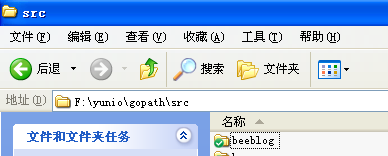
\includegraphics[width=7cm]{13.1.gopath2.png}
   \label{図13.2}
   \caption{ワーキングディレクトリは\$gopath/srcの下にあります}
\end{figure}


